% Options for packages loaded elsewhere
\PassOptionsToPackage{unicode}{hyperref}
\PassOptionsToPackage{hyphens}{url}
\documentclass[
]{article}
\usepackage{xcolor}
\usepackage[margin=1in]{geometry}
\usepackage{amsmath,amssymb}
\setcounter{secnumdepth}{-\maxdimen} % remove section numbering
\usepackage{iftex}
\ifPDFTeX
  \usepackage[T1]{fontenc}
  \usepackage[utf8]{inputenc}
  \usepackage{textcomp} % provide euro and other symbols
\else % if luatex or xetex
  \usepackage{unicode-math} % this also loads fontspec
  \defaultfontfeatures{Scale=MatchLowercase}
  \defaultfontfeatures[\rmfamily]{Ligatures=TeX,Scale=1}
\fi
\usepackage{lmodern}
\ifPDFTeX\else
  % xetex/luatex font selection
  \setmainfont[]{Segoe UI}
  \setmonofont[]{Consolas}
\fi
% Use upquote if available, for straight quotes in verbatim environments
\IfFileExists{upquote.sty}{\usepackage{upquote}}{}
\IfFileExists{microtype.sty}{% use microtype if available
  \usepackage[]{microtype}
  \UseMicrotypeSet[protrusion]{basicmath} % disable protrusion for tt fonts
}{}
\makeatletter
\@ifundefined{KOMAClassName}{% if non-KOMA class
  \IfFileExists{parskip.sty}{%
    \usepackage{parskip}
  }{% else
    \setlength{\parindent}{0pt}
    \setlength{\parskip}{6pt plus 2pt minus 1pt}}
}{% if KOMA class
  \KOMAoptions{parskip=half}}
\makeatother
\usepackage{longtable,booktabs,array}
\newcounter{none} % for unnumbered tables
\usepackage{calc} % for calculating minipage widths
% Correct order of tables after \paragraph or \subparagraph
\usepackage{etoolbox}
\makeatletter
\patchcmd\longtable{\par}{\if@noskipsec\mbox{}\fi\par}{}{}
\makeatother
% Allow footnotes in longtable head/foot
\IfFileExists{footnotehyper.sty}{\usepackage{footnotehyper}}{\usepackage{footnote}}
\makesavenoteenv{longtable}
\usepackage{graphicx}
\makeatletter
\newsavebox\pandoc@box
\newcommand*\pandocbounded[1]{% scales image to fit in text height/width
  \sbox\pandoc@box{#1}%
  \Gscale@div\@tempa{\textheight}{\dimexpr\ht\pandoc@box+\dp\pandoc@box\relax}%
  \Gscale@div\@tempb{\linewidth}{\wd\pandoc@box}%
  \ifdim\@tempb\p@<\@tempa\p@\let\@tempa\@tempb\fi% select the smaller of both
  \ifdim\@tempa\p@<\p@\scalebox{\@tempa}{\usebox\pandoc@box}%
  \else\usebox{\pandoc@box}%
  \fi%
}
% Set default figure placement to htbp
\def\fps@figure{htbp}
\makeatother
\ifLuaTeX
  \usepackage{luacolor}
  \usepackage[soul]{lua-ul}
\else
  \usepackage{soul}
\fi
\setlength{\emergencystretch}{3em} % prevent overfull lines
\providecommand{\tightlist}{%
  \setlength{\itemsep}{0pt}\setlength{\parskip}{0pt}}
% LaTeX transcription of published v1.1.0, not its original authoring source.
% Source SHA256 D894D75945DC94E819BA5EB5F6ECF6300D6596CF43F94444990D4DD4AA7A9A6C.
\usepackage{newunicodechar}
\newunicodechar{⊂}{\ensuremath{\subset}}
\newunicodechar{∈}{\ensuremath{\in}}
\raggedbottom
\usepackage{caption}
\captionsetup{labelformat=empty}
\AtBeginEnvironment{longtable}{\setlength{\parskip}{0pt}}
\usepackage{bookmark}
\IfFileExists{xurl.sty}{\usepackage{xurl}}{} % add URL line breaks if available
\urlstyle{same}
\hypersetup{
  pdftitle={Genesis on the GPU},
  hidelinks,
  pdfcreator={LaTeX via pandoc}}

\title{Genesis on the GPU}
\usepackage{etoolbox}
\makeatletter
\providecommand{\subtitle}[1]{% add subtitle to \maketitle
  \apptocmd{\@title}{\par {\large #1 \par}}{}{}
}
\makeatother
\subtitle{Hardware-Seeded Initialization and Verified Agreement in a
Geometric World}
\author{}
\date{}

\begin{document}
\maketitle

Devon A. Generally\\
MetaCortex Dynamics LLC\\
ORCID 0009-0004-8164-2159

Version 1.1.0 • 22 October 2026\\
Status through 22 October 2026 at 21:21 ET • Second-step update prepared
22 October 2026

Published predecessor: https://doi.org/10.5281/zenodo.23580914

This version:
\href{https://doi.org/10.5281/zenodo.23584296}{\ul{https://doi.org/10.5281/zenodo.23584296}}

\section{Abstract}\label{abstract}

We report hardware-situated genesis on an NVIDIA GeForce RTX 3070 and
subsequent GPU conformance of the first-tick specification on its frozen
V1/V2 vectors. A captured junction transition supplies the locus of a
distinction on 480 flags and 720 overlap pairs. From an all-NO
predecessor, twelve flags at the event junction read THIS; the witness
contains 708 SAME readings and twelve \nolinkurl{NOT_SAME} walls. The
J17 world has committed two links: genesis and a second link that leaves
the field unchanged. Separately, four execution obligations are
\nolinkurl{IF_THEN} for frozen V1/V2, with independent-builder
comparison discharged for those vectors. V1/V2 used empty route lists;
the second link exercised propagation and DRC(iv) on twelve admitted
routes. {[}2, 3, 8, 9{]}

The verification target is whether event, incidence, field, agreement
witness and predecessor bindings agree under the governing relations.
This paper distinguishes inspected genesis artifacts from the later
promoted results supplied in the current handoff. The V1/V2 comparison
joins hand derivation, GPU output and a separate builder's realization;
independence is builder-attested and output equality locally witnessed.
The retained genesis subset permits direct artifact checks, but is not a
complete public GPU replay release. \nolinkurl{O_exec} remains nonempty
because JTP obligation construction remains MAYBE. {[}6, 8{]}

\begin{figure}
\centering
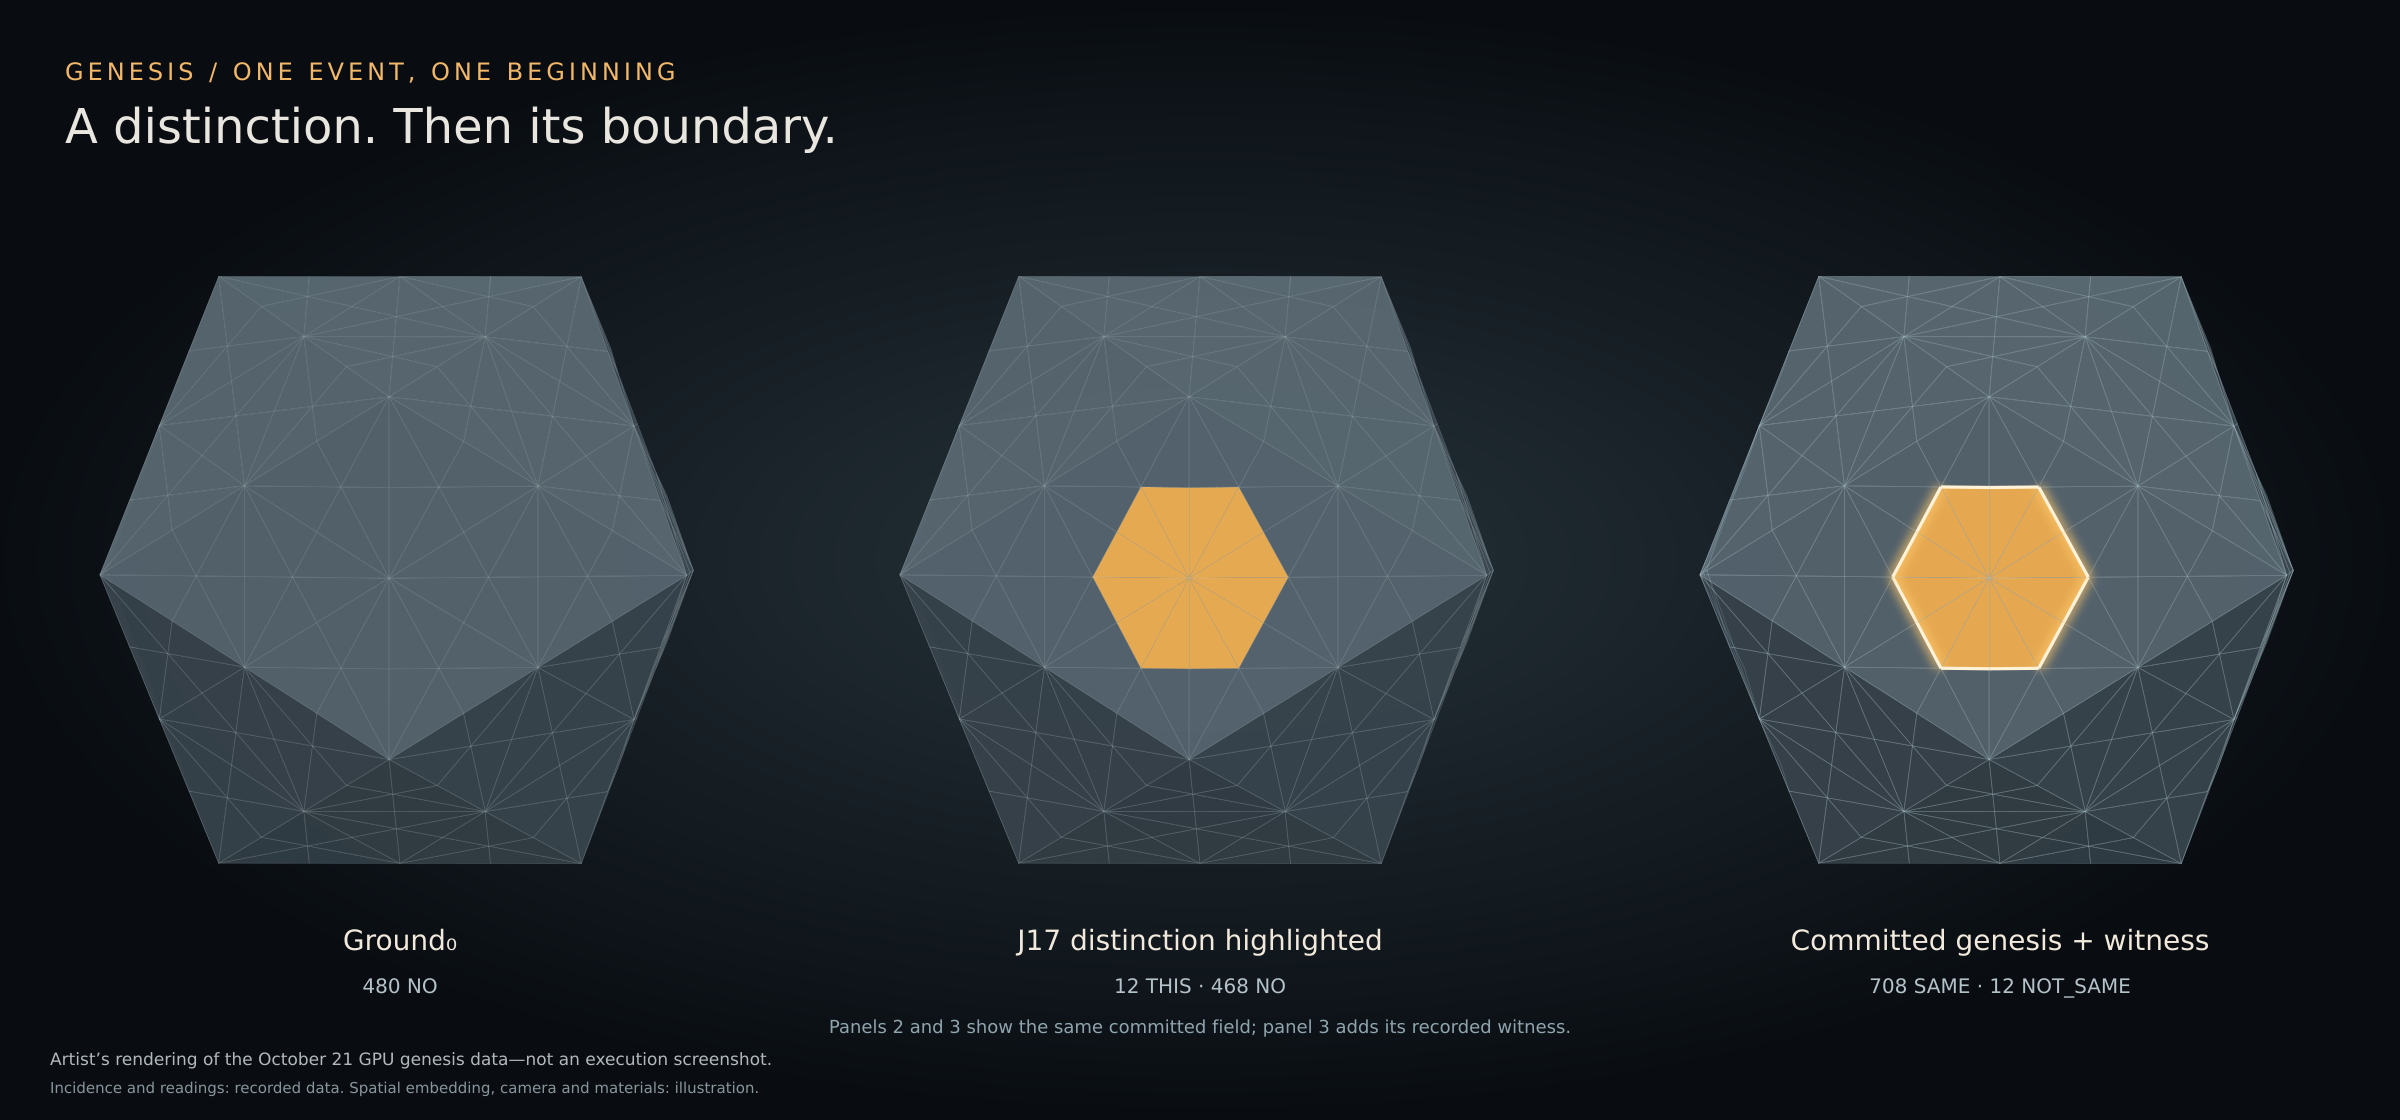
\includegraphics[width=6in,height=\textheight,keepaspectratio]{./media/image1.png}
\caption{Figure 1. Ground₀, the genesis field, and its witness overlay.
The latter two views depict the same committed state. Artist's rendering
of the October 21 GPU genesis data---not an execution screenshot.
Coordinates are illustrative; incidence and markings come from retained
data.}
\end{figure}

\section{1 Carrier and event situated
initialization}\label{carrier-and-event-situated-initialization}

The program's carrier is specified through incidence. The retained
hardware motif table identifies twelve domains, thirty junctions and
twenty witness faces. Its dual incidence has the familiar twelve-face,
thirty-edge, twenty-corner counts of a Megaminx. The extracted carrier
payload describes a combinatorial icosidodecahedron obtained by
rectification of the dodecahedral--icosahedral dual pair. These
descriptions refer to related incidence objects; their counts must not
be interchanged. {[}1--3{]}

The refined flag-world has 42 sites, 120 edges and 80 triads. A flag is
an incident triple f = (s, e, t), with site s belonging to edge e and
edge e belonging to triad t. Six flags per triad give 480 flags. The
overlap witness records 240 pairs of each of the three kinds δ, γ and τ,
for 720 pairs in total. A pair differs in exactly one component of its
flag triple. {[}1, 2{]}

No XYZ coordinate embedding enters the recorded semantic identity. The
figures embed incidence for presentation; their rendered distances and
angles do not define the world's relations. The current handoff records
the seated hardware frame as constitutional and chiral, with seating
stabilizer \{id\} among the 120 symmetries, verified twice. Grounding
refers to the real-world seating, not a direction. It also states that a
flag is a cell whose reading is its state, and that occurrences are
located by their own incidence coordinates rather than their type's
seat. These settled bindings are cited without re-derivation. {[}1, 8{]}

\subsection{Ground and the captured
locus}\label{ground-and-the-captured-locus}

Write F for the finite flag set and q₀ : F → \{NO, THIS\} for the
initial field. Ground₀ has q₀(f) = NO for every f. NO is a determined
field reading. It is not missing input, UNREAD, or MAYBE. Ground₀ is
retained as exact bytes with its own SHA-256 identity. {[}1, 2{]}

The captured 132-byte protocol record names Junction 17 in its header.
The run binds that junction to the corridor between domains 4 and 9,
represented in the field as C:HW\_04\textbar{}\nolinkurl{HW_09.} Its
payload byte is not used to index a flag or select an address. Given
that bound event locus j, the genesis field is: {[}2, 3{]}

\begin{quote}
q₁(f) = THIS if site(f) = j; otherwise q₁(f) = NO.
\end{quote}

Exactly twelve flags have site j. The resulting field therefore contains
twelve THIS and 468 NO readings. This is a conditional determination
from the captured event and the admitted incidence. It does not predict
which physical junction will emit the first event. The event supplies
that input; identifier ordering supplies no additional selection.
{[}2{]}

{\def\LTcaptype{none} % do not increment counter
\begin{longtable}[]{@{}
  >{\raggedright\arraybackslash}p{(\linewidth - 4\tabcolsep) * \real{0.3333}}
  >{\raggedright\arraybackslash}p{(\linewidth - 4\tabcolsep) * \real{0.3333}}
  >{\raggedright\arraybackslash}p{(\linewidth - 4\tabcolsep) * \real{0.3333}}@{}}
\toprule\noalign{}
\begin{minipage}[b]{\linewidth}\raggedright
\textbf{Object}
\end{minipage} & \begin{minipage}[b]{\linewidth}\raggedright
\textbf{Recorded size}
\end{minipage} & \begin{minipage}[b]{\linewidth}\raggedright
\textbf{Function}
\end{minipage} \\
\midrule\noalign{}
\endhead
\bottomrule\noalign{}
\endlastfoot
Hardware motif & 12 domains · 30 junctions · 20 faces & Binds event
locus and carrier incidence \\
Refined carrier & 42 sites · 120 edges · 80 triads & Supports flag
triples \\
Field & 480 readings & Records the realized distinction \\
Witness & 720 overlap readings & Records agreement and walls \\
\end{longtable}
}

\section{2 Agreement and the committed
witness}\label{agreement-and-the-committed-witness}

For each retained overlap pair (f, f′), the witness reads SAME when
q₁(f) and q₁(f′) are equal, and \nolinkurl{NOT_SAME} when they differ.
In this snapshot the field alphabet is \{NO, THIS\}; the witness
alphabet is \{SAME, NOT\_SAME\}\nolinkurl{.} These are distinct typed
readings. The field's NO must not be confused with a failed agreement
reading. {[}1, 2{]}

{\def\LTcaptype{none} % do not increment counter
\begin{longtable}[]{@{}
  >{\raggedright\arraybackslash}p{(\linewidth - 6\tabcolsep) * \real{0.2500}}
  >{\raggedright\arraybackslash}p{(\linewidth - 6\tabcolsep) * \real{0.2500}}
  >{\raggedright\arraybackslash}p{(\linewidth - 6\tabcolsep) * \real{0.2500}}
  >{\raggedright\arraybackslash}p{(\linewidth - 6\tabcolsep) * \real{0.2500}}@{}}
\toprule\noalign{}
\begin{minipage}[b]{\linewidth}\raggedright
\textbf{Overlap kind}
\end{minipage} & \begin{minipage}[b]{\linewidth}\raggedright
\textbf{SAME}
\end{minipage} & \begin{minipage}[b]{\linewidth}\raggedright
\textbf{\nolinkurl{NOT_SAME} walls}
\end{minipage} & \begin{minipage}[b]{\linewidth}\raggedright
\textbf{Total}
\end{minipage} \\
\midrule\noalign{}
\endhead
\bottomrule\noalign{}
\endlastfoot
δ & 228 & 12 & 240 \\
γ & 240 & 0 & 240 \\
τ & 240 & 0 & 240 \\
All kinds & 708 & 12 & 720 \\
\end{longtable}
}

All twelve walls are δ overlaps, where the site component changes. They
are exactly the overlaps crossing between the twelve THIS flags and the
remaining NO flags. Relative to the all-NO predecessor, the transition
opens twelve walls and discharges none; 708 overlap readings remain
unchanged. The wall set is derived from the complete field and incidence
rather than supplied as a separate placement list. {[}1, 2{]}

Run 018 reports one committed genesis chain link, binding the event
record, field, witness and predecessor. Its commit support distinguishes
the earlier construction stages, which have no
\nolinkurl{COMMITTED_GENESIS} fact, from the publication stage, which
has exactly one. The later readout reconstitutes that same genesis
record to retain its dependency; this is not an additional worldline
link. {[}2{]}

\subsection{Distance across the predecessor
relation}\label{distance-across-the-predecessor-relation}

The junction readout compares the committed field with Ground₀. For a
junction j, let I(j) contain each flag incident to j through its site,
edge or triad. Because site ⊂ edge ⊂ triad within a flag, this union
reduces to triad containment. Each changed flag is counted once: {[}2{]}

\begin{quote}
d(j; q₀, q₁) = \textbar\{ f ∈ I(j) : q₀(f) ≠ q₁(f) \}\textbar.
\end{quote}

The retained encoding represents each edit by one THIS entry.
Cardinalities in this paper are observations of those entries. They are
not identifier magnitudes. J17 has distance twelve. Its four
neighbouring junctions in W12 and W13 each have distance four; the
remaining 25 junctions have distance zero (domains are not ranked by the
readout law). This explains why ``flags changed at a junction'' must
include incident support, rather than only flags whose site equals that
junction. {[}2{]}

Within each of J17's two witness faces, the distances are (4, 12, 4).
The face terms coexist in the carrier, while their distances depend on
two successive fields. Thus the readout uses both incidence and
genealogy. Nothing in this definition requires treating the drawing as
Euclidean space or Worldline as a Euclidean axis.

\section{3 The incircle result and the role
correspondence}\label{the-incircle-result-and-the-role-correspondence}

The Perfect-Square Incircle Law supplies a precise mathematical result.
For a primitive Pythagorean triple with Euclid parameters m
\textgreater{} n \textgreater{} 0, coprime and of opposite parity, the
side lengths are a = m² − n², b = 2mn and c = m² + n². The inradius is
{[}5{]}

\begin{quote}
r = (a + b − c)/2 = n(m − n),\\
so incircle area = π{[}n(m − n){]}².
\end{quote}

Area π requires n(m − n) = 1. Positive integrality gives n = 1 and m =
2, hence the unique primitive triple 3--4--5. With semiperimeter six,
its vertex tangent lengths are 6−5 = 1, 6−4 = 2 and 6−3 = 3. The
right-angle vertex has tangent length one. The paper's
constitutive-square theorem characterizes the square formed there by the
vertex, adjacent tangency points and incenter. {[}5, §§3--6{]}

The incircle supplies the reading under which the capability-forced
ranks are G, F and S. The current handoff states that the incircle is a
projection, G occupies the right angle, and the operative metric belongs
to the §6.1 readout as \nolinkurl{d_G}, not to a ProjectionShell
refinement. The promoted S/F binding assigns rank 1 to G, rank 2 to F
and rank 3 to S. The edit observations (4, 12, 4) are therefore read
through that governed correspondence; this paper does not identify them
with side lengths of a rendered triangle. {[}5, 8{]}

\subsection{What the genesis records
establish}\label{what-the-genesis-records-establish}

Run 018 binds the distance and witness-face readout laws by full hash.
Its face readouts leave G at MAYBE when the minimum is tied; all twenty
recorded faces have tied minima in this checkpoint. Run 019 applies the
subsequently promoted S/F binding and records J17 as S on W12 and W13.
The supporting terms are
GOES\_WITH(SF\_FACE\_ROLE,W\_12,J\_17,\nolinkurl{S}) and
GOES\_WITH(SF\_FACE\_ROLE,W\_13,J\_17,S)\nolinkurl{.} The two
neighbouring minima are not assigned G or F by a tie-breaker. {[}2, 3{]}

The current handoff confirms the promoted role law and the J17 result.
On W12 and W13, J17 has unique rank 3 and therefore reads S. A tie among
the other vertices is not a stop for a cell whose own rank is unique.
The exact law identities remain in Appendix A. Attaching their full
texts to the publication package makes this correspondence inspectable
by an external verifier; it does not reopen their promotion. {[}8{]}

\begin{figure}
\centering
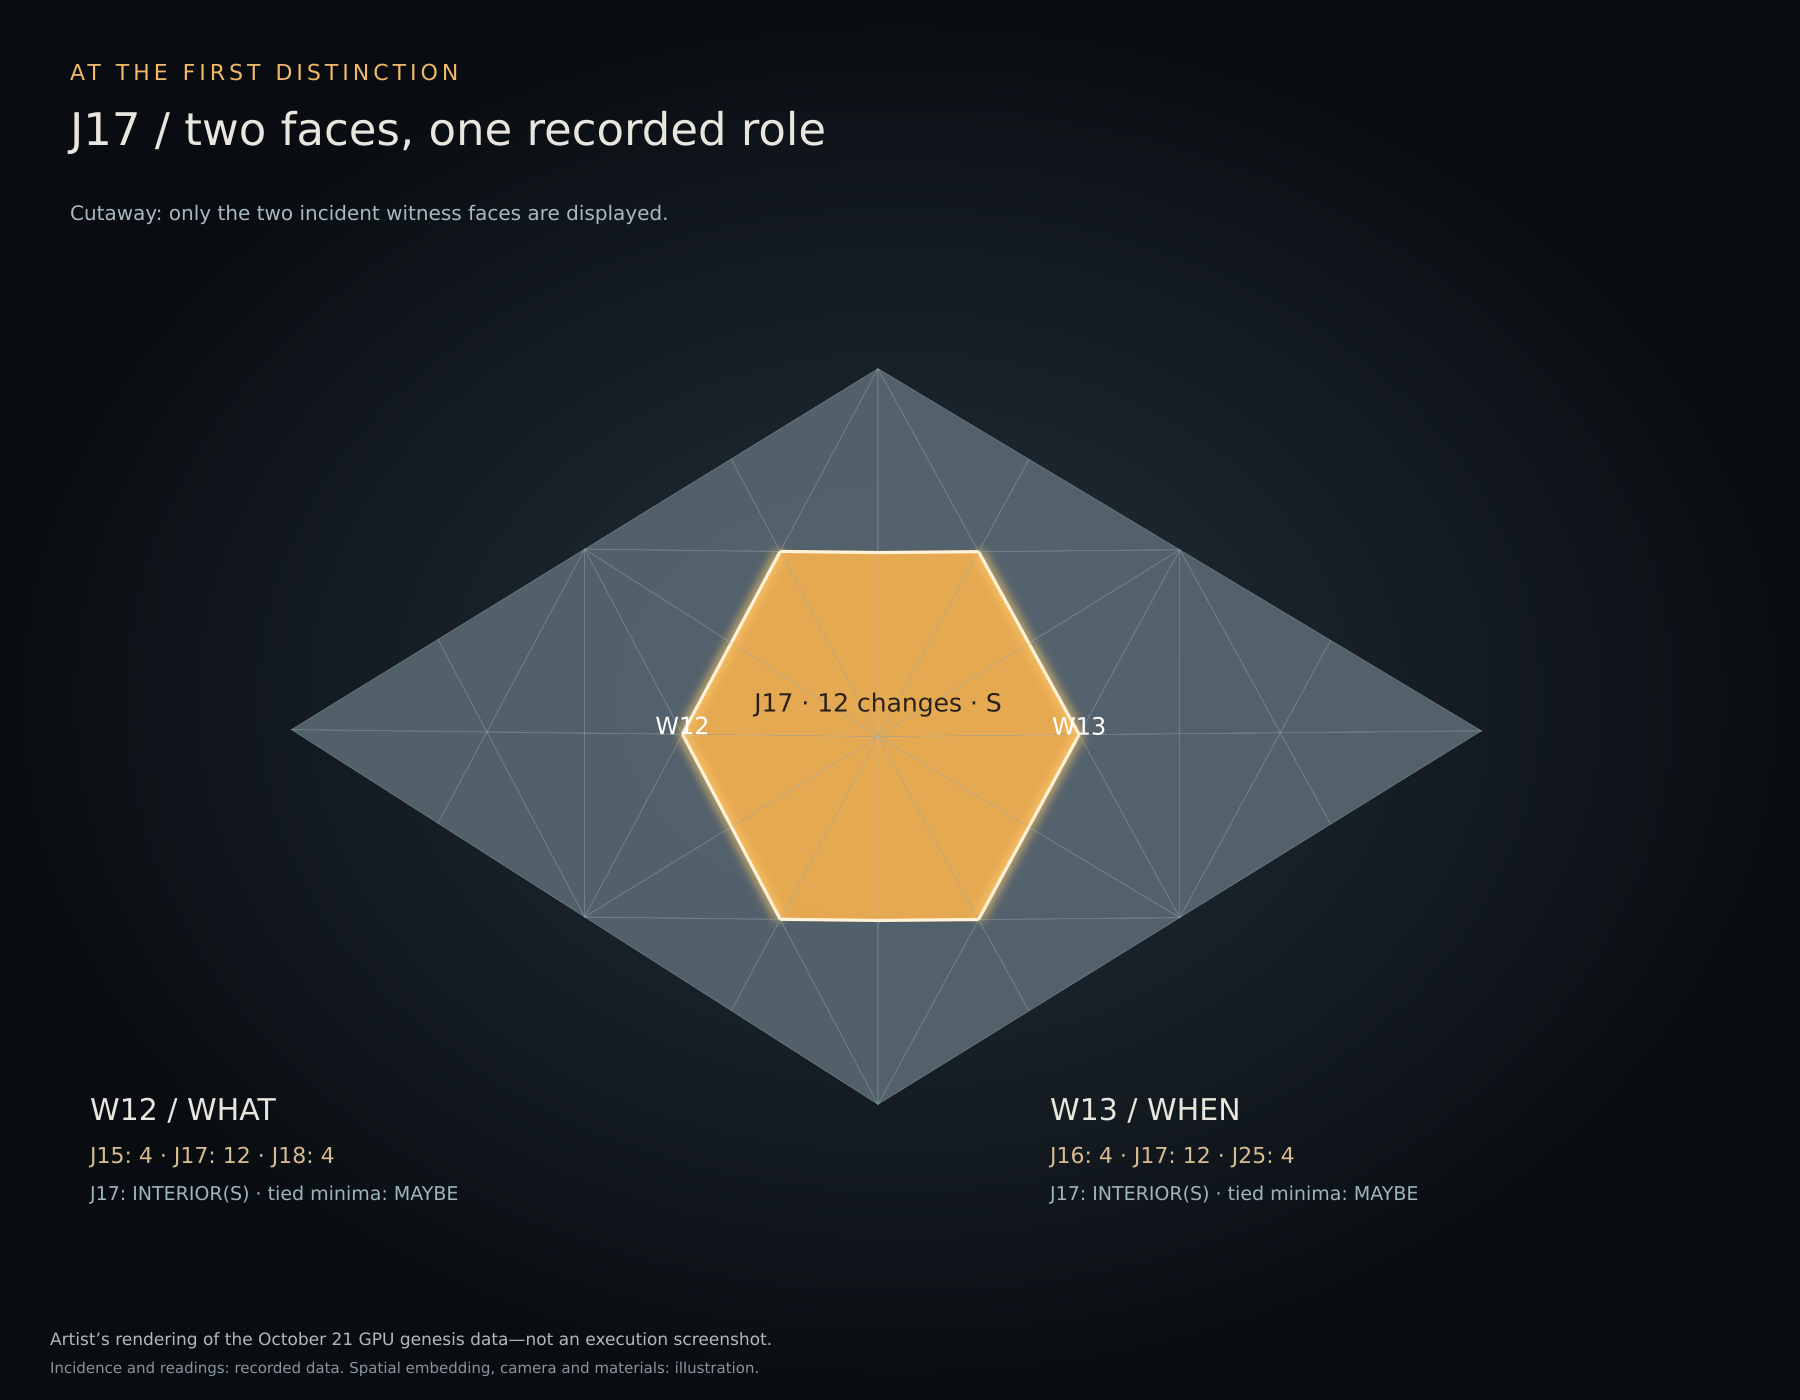
\includegraphics[width=3.5in,height=2.72222in]{./media/image2.png}
\caption{Figure 2. J17 and its two incident witness faces. Artist's
rendering of the October 21 GPU genesis data---not an execution
screenshot. Rendered lengths do not supply the role law.}
\end{figure}

\section{4 Execution semantics and observed
scope}\label{execution-semantics-and-observed-scope}

Programming with Geometry defines the five phases of snapshot, cell
evaluation, route propagation, runtime governance and simultaneous
commit. Active cells read one immutable snapshot; routes are standing
incidence relations. Its fixed-program condition remains in force. For
the flag-world markers, the current handoff explicitly rejects a
program/state dichotomy: flags are cells, and their readings are state.
The second-step construction inspected the candidate overlap routes and
withheld cells without complete placement evidence. The admitted program
and its twelve routes are reported in §4A; this does not establish
execution of all 1,440 candidate routes. {[}4, 8{]}

Paper B's \nolinkurl{HOST_ORDER_ERASURE} result is conditional on valid
schedules and the stated semantic functions. Its reported 70-vector
conformance corpus and 71 byte-identical artifacts concern mal-fabric
v0.3.0. They are inherited framework evidence, not 70 genesis tests or a
proof that this particular GPU run implements every fabric law. {[}4,
§§9--10, 12{]}

Run 018 identifies the GPU as an RTX 3070. It records .mal application
consequences executed by a generic CUDA evaluator, with host
parsing/lowering, custody and observation serialization, plus generic
GPU hash dispatch. Its source, executable and stage identities are
retained in the run record. The record's source-bound scope claim is
distinct from a new audit of all listed binaries: many of those bytes
are outside the artist subset supplied here. {[}2{]}

Run 019 records 720 placed, admitted and evaluated snapshot comparators
and no second world-transition receipt. That is the genesis-era
checkpoint. The updated handoff records the subsequent first-tick
CONFORM result as \nolinkurl{IF_THEN} for V1/V2, promoted on October 22,
with run record prefix 6089FDC4. The discharge map marks
\nolinkurl{O_SOURCE_DERIVED_LOWERING}, \nolinkurl{O_GPU_STEP_EXECUTION},
\nolinkurl{O_COMMIT} and \nolinkurl{O_VECTOR_CONFORMANCE}
\nolinkurl{IF_THEN} for those frozen vectors. Both vectors used empty
route lists and propagation returned NIL; DRC(iv) was not exercised.
These results do not constitute the J17 world's second step. The second
step (§4A) subsequently exercised non-empty propagation. {[}3, 8, 9{]}

\subsection{Verification performed for this
paper}\label{verification-performed-for-this-paper}

The accompanying read-only checker rehashed all thirty entries in the
supplied SHA256SUMS file. It checked the exact 480-flag field domain,
the all-NO predecessor, the J17 marking rule, all 720 unique overlap
pairs and every agreement reading. It recomputed all thirty junction
edit counts from the retained fields and incident support, checked all
twenty tied-minimum face readouts, and checked that the committed record
contains the supplied field. Every check passed. {[}6{]}

These checks establish internal consistency of retained artifacts. They
do not rerun a native body, authenticate the original hardware capture
independently, or reproduce the GPU executor. The checker is
supplementary publication verification and adds no execution credit.

\subsection{Independent construction
evidence}\label{independent-construction-evidence}

Three verification scopes must remain distinct. Run 018 reports
source/support checks and direct checks of distances and face outputs.
The ref012 builder comparison reports 65/65 full-set agreements for the
carrier construction and genesis quantities, with index prefix
1FA1397F\ldots3FD79. The later
\nolinkurl{RECORD_INDEPENDENT_BUILDER_COMPARISON_001} discharges the
independent comparison obligation for frozen V1/V2: hand derivation, GPU
and Claude's realization agree byte for byte. Its record prefix is
99CC2107, realization \nolinkurl{first_tick_ib.py} prefix E02C90DE and
bundle prefix 99561FDE. Independence is builder-attested; equality is
locally witnessed. The handoff reports these current results; manuscript
preparation did not independently rerun either builder. {[}2, 8{]}

\section{4A The second step and its unchanged
field}\label{a-the-second-step-and-its-unchanged-field}

The supplied run account reports the J17 world's second step on 22
October 2026 across three governed runs. Before link 2, the available
readout is over (Ground₀, g₁), the only successive field pair then
committed. Earlier planning language that read the successor before
producing it was circular and is withdrawn; the account reports that
nothing executed under it. New run identities are cited in {[}9{]};
their bytes were not supplied in this revision session.

\subsection{Marker location}\label{marker-location}

The 480 THIS×WHAT occurrences are located by their own flag coordinates.
Twelve are admitted: J17's four flags on W12 and W13, where it has
unique rank 3 and reads S, and two flags for each of the four
neighbouring junctions on its outer witness face, where the neighbour
alone has rank 3 in a (4, 0, 0) readout. No unique-rank F occurrence
appears. {[}3, 8--10{]}

{\def\LTcaptype{none} % do not increment counter
\begin{longtable}[]{@{}
  >{\raggedright\arraybackslash}p{(\linewidth - 4\tabcolsep) * \real{0.3333}}
  >{\raggedright\arraybackslash}p{(\linewidth - 4\tabcolsep) * \real{0.3333}}
  >{\raggedright\arraybackslash}p{(\linewidth - 4\tabcolsep) * \real{0.3333}}@{}}
\toprule\noalign{}
\begin{minipage}[b]{\linewidth}\raggedright
\textbf{Occurrence class}
\end{minipage} & \begin{minipage}[b]{\linewidth}\raggedright
\textbf{Count}
\end{minipage} & \begin{minipage}[b]{\linewidth}\raggedright
\textbf{Readout and location}
\end{minipage} \\
\midrule\noalign{}
\endhead
\bottomrule\noalign{}
\endlastfoot
Admitted & 12 & Unique rank 3, S; marker capability \{G, S\} \\
Tied own rank & 108 & 84 on 14 untouched faces; 24 on six affected
faces \\
Outside face-readout scope & 360 & Six flags in each of sixty CCD
triads \\
Total & 480 & All marker occurrences accounted for \\
\end{longtable}
}

The 108 tied occurrences comprise all six flags on each of fourteen
untouched faces, plus four tied-vertex flags on each of six affected
faces. The retained genesis readouts contain fourteen (0, 0, 0) faces,
four permutations of (4, 0, 0), and two permutations of (4, 12, 4).
These counts correct the supplied insertion's description of eighteen
untouched faces. During preparation of this revision, the retained
genesis face-readout data were checked for these counts. The subsequent
document review confirmed arithmetic and agreement between the DOCX and
PDF. A tied vertex is a boundary location requiring both dimensions'
capabilities; the marker carries \{G, S\} only. The cited requirement
withholds candidates missing placement evidence, without selecting a
location on the author's behalf. The sixty CCD triads are outside the
promoted face readout's scope. {[}1, 9, 10{]}

\subsection{Route topology}\label{route-topology}

Each admitted marker has three overlap partners. Its δ partner is tied
and withheld; its τ partner lies in an unlocated CCD triad; its γ
partner is admitted. Of the 36 routes from twelve admitted markers,
twelve reach comparators with both operands admitted and 24 reach
comparators missing one located operand. The supplied run reports those
24 joins as \nolinkurl{NOT_SAME} under the complete operator-role
topology check. Applying the placement requirement to the comparators as
well as the markers leaves six comparators, twelve markers and twelve
routes, with no open join. All eight design-rule conditions are reported
\nolinkurl{IF_THEN} on that admitted program. {[}9, 10{]}

\section{4A Execution and the boundary of the fixed
point}\label{a-execution-and-the-boundary-of-the-fixed-point}

\nolinkurl{STEP_FABRIC} ran over g₁ on the admitted program. Each of the
six comparators read a vertex's two flags within one face: J17's pairs
were THIS/THIS and the neighbours' outer-face pairs were NO/NO. All six
returned SAME. No admitted cell writes a flag. The successor field
equals g₁, with 708 SAME readings, twelve retained walls, zero opened
and zero discharged; the receipt reads NO. Link 2 was committed on the
GPU. The readout over (g₁, g₂) is (0, 0, 0) on all twenty faces, without
a tie-break. {[}9{]}

\subsection{What the result
establishes}\label{what-the-result-establishes}

Non-empty route propagation and DRC(iv) have their own bounded execution
result: twelve admitted routes at link 2. This extends the reported
execution evidence beyond empty-route cases; it does not retroactively
change the frozen V1/V2 vectors or establish all possible route
topologies. {[}8, 9{]}

The committed field is unchanged by this admitted read-only program: g₂
= g₁. In that precise field-update sense, the tested program has a fixed
point at g₁. The worldline nevertheless advances by one committed link.
The supplied finding names this result \nolinkurl{FIXED_POINT.} {[}9,
11{]}

An unchanged field does not establish an unchanged admission on tick 3.
Placement uses predecessor-relative edit counts, and the newly available
pair (g₁, g₂) gives tied zeros everywhere. Re-admission from that pair
therefore cannot be asserted to recover the twelve-marker program
without a separate governing persistence rule. Reapplying a retained
read-only program would preserve the field, but retention and
re-admission are distinct claims. No tick-3 invocation is reported here.

\subsection{Next event and limits}\label{next-event-and-limits}

The next planned field update is a second captured junction transition
from the hardware lane, bound to its locus as the first was.
Constructing its retained transition obligations and satisfying the
hardware board-receipt boundary precede the proposed link 3. The
supplied finding identifies this as the standing external-input path;
this paper does not infer from one read-only program that every possible
endogenous field change is impossible. {[}8, 11{]}

No new placement ruling is reported for link 2: missing-evidence
withholding applies to tied markers, out-of-scope CCD markers and
comparators without a located operand. A second event may alter edit
counts, break some ties or create others. It does not by itself
guarantee more admitted cells or any writer. Extending the readout to
all eighty triads remains a proposal. The supplied finding reports tied
four-edit readings for the neighbouring junction and domain at J17's
four CCD triads; that is not an executed extension of the readout.
{[}10, 11{]}

\section{5 External verification and remaining
work}\label{external-verification-and-remaining-work}

The public objective is verification. A third party should be able to
identify the frozen inputs, reproduce the relevant construction, compare
complete outputs and report a specific agreement or discrepancy.
Contribution to the implementation is not a prerequisite.

\subsection{Two reproducibility
levels}\label{two-reproducibility-levels}

Genesis artifact verification uses
\nolinkurl{genesis_verification_supplement_001.zip} {[}1, 6{]}: verify
its hash lists, reconstruct the field and overlap relations, and compare
exact readings. Its \nolinkurl{verify_genesis.py} uses Python's standard
library; invoke it with the extracted bundle directory as argument. The
result is artifact consistency, not GPU replay. The public 901-file
repository subset at 60340c61 is a separate package with a separate
checker. The deposit report records an independent-checker pass, but no
execution of the repository verify.mjs in that session; coverage
equivalence is unestablished.

GPU execution reproduction needs a release containing the exact source
closure, lowering tools, generic evaluator, hash implementation, stage
inputs, canonical encoders and recorded command lines. Run 018
identifies these objects and its stage order, but identification is not
delivery. A public kit must include the bytes or stable retrievable
references and distinguish semantic identities from hashes of serialized
observation files. Reproduction on AMD, Apple Silicon or another NVIDIA
target remains a separate verification result; this paper reports no
cross-device run.

\subsection{Checks for the public kit}\label{checks-for-the-public-kit}

The kit should expose the exact frozen V1/V2 inputs, expectations and
three-route comparison, together with the genesis-specific field,
witness and predecessor checks. Empty-route success must be labelled
explicitly. Non-empty propagation and DRC(iv) have their own reported
result from the J17 second step (§4A); the kit should expose it
separately from V1/V2. Proposed additional rejection checks should be
labelled as such rather than silently counted as executed evidence.
{[}8{]}

A reusable event interface must bind protocol bytes, validated locus,
incidence and field identity. Each new source needs its own provenance
and locus correspondence; a timestamp alone supplies no carrier
junction.

\subsection{Publication completion
items}\label{publication-completion-items}

{\def\LTcaptype{none} % do not increment counter
\begin{longtable}[]{@{}
  >{\raggedright\arraybackslash}p{(\linewidth - 2\tabcolsep) * \real{0.5000}}
  >{\raggedright\arraybackslash}p{(\linewidth - 2\tabcolsep) * \real{0.5000}}@{}}
\toprule\noalign{}
\begin{minipage}[b]{\linewidth}\raggedright
\textbf{Evidence item}
\end{minipage} & \begin{minipage}[b]{\linewidth}\raggedright
\textbf{Status through 21:21 ET}
\end{minipage} \\
\midrule\noalign{}
\endhead
\bottomrule\noalign{}
\endlastfoot
Governing law texts & Promoted; attach exact texts for external
verification \\
Frozen V1/V2 & Four \nolinkurl{O_exec} items \nolinkurl{IF_THEN}; empty
routes only \\
Independent V1/V2 comparison & DISCHARGED; builder-attested
independence \\
J17 second step & Link 2 committed; twelve routes; unchanged field
(§4A) \\
JTP obligation construction & MAYBE; \nolinkurl{O_exec} remains
nonempty \\
Public evidence and repository home & 901 files at
\nolinkurl{mal-fabric/flag_world_001_first_tick/} (60340c61); tree ids
preserved \\
Public replay kit & Not released \\
\end{longtable}
}

Next: construct the junction-transition obligations for a second
captured event, its field edit and link 3. The hardware board-receipt
obligation gates frame emission. Second-step records were uncommitted at
the supplied cutoff and are not part of the earlier 60340c61 release.
{[}8, 9{]}

\section{References and exact evidence
locators}\label{references-and-exact-evidence-locators}

{[}1{]} Genesis artist bundle 001, packaged 22 October 2026; retained
unchanged in \nolinkurl{genesis_verification_supplement_001.zip.}
Includes README.md, MANIFEST.json, SHA256SUMS.txt,
\nolinkurl{PACKAGING_CHECKS.json} and carrier/run data. The separate
901-file evidence subset is public at mal-fabric
\nolinkurl{flag_world_001_first_tick/} (commit 60340c61; tree identities
preserved). A replay kit --- source closure, evaluator, encoders,
command lines --- is not released.

{[}2{]} \nolinkurl{RUN_RECORD_018_GPU_SELF_WITNESS_AND_G_READOUT.} 21
October 2026. \nolinkurl{gpu_self_witness_018/RUN_RECORD_018.json.}
Sections \nolinkurl{governing_bindings}, realization, reproducibility,
genesis, readout and \nolinkurl{independent_checks.} Associated field,
witness, receipt and committed.genesis.json are in the same directory.

{[}3{]} \nolinkurl{s_f_binding_019/RUN_RECORD_019.json.} 21 October
2026. Sections authority, roles, \nolinkurl{snapshot_reading_counts},
receipts and \nolinkurl{source_contacts.} Hardware locus:
\nolinkurl{jtp_locus_017/inputs/frame.json} and frame.json.source.bin;
incidence sources under \nolinkurl{hardware_carrier_012/.}

{[}4{]} D. A. Generally, Programming with Geometry: Synchronous Spatial
Execution and Host-Order Erasure in Operator-Witness Fabrics.
\nolinkurl{Programming_with_Geometry_Paper_B_FINAL.docx}, inspected
copy. Static companion: DOI 10.5281/zenodo.22677712. Fabric releases:
10.5281/zenodo.22678128, 10.5281/zenodo.22711890 and
10.5281/zenodo.22713736. Paper B records v0.3.0 promotion at commit
\nolinkurl{98289c348421943ab0e440d45ec1d7e7cbbbc2b2.}

{[}5{]} Generally, Devon A., The Perfect-Square Incircle Law: Incircle
Areas of Primitive Pythagorean Triangles.
\nolinkurl{Perfect_Square_Incircle_Law.docx}, inspected copy, §§3--6.
Public record supplied by the author:
https://zenodo.org/records/20946692. Equality between this inspected
document and the published bytes has not been checked for this paper.

{[}6{]} \nolinkurl{verify_genesis.py} and verification.json, deposited
in \nolinkurl{genesis_verification_supplement_001.zip}; published with
the predecessor paper at DOI 10.5281/zenodo.23580914, as reported by the
author. Standard-library read-only artifact check; no runtime or
hardware execution. Thirty file hashes, 480 field readings, 720
overlaps, thirty junction distances and twenty face readouts checked.

{[}7{]} Author's October 21 genesis account supplied in the
conversation. Historical narrative only; the October 22 handoff {[}8{]}
controls execution scope, with repository status superseded by {[}12{]}.

{[}8{]} \nolinkurl{HANDOFF_FLAG_WORLD_FIRST_TICK_2026-10-21.md}, status
through 22 October 2026 at 21:21 ET. Updated identity supplied by the
author:
\nolinkurl{b9618192a5d0f8d4bc3e4b7ecaf44efd45e6ddabbd6aaa33563ea9de6f704867.}
Updated bytes were not supplied in this revision session. The inspected
earlier 18:00 handoff remains genealogy; second-step claims here follow
the supplied insertion and record locators {[}9--11{]}.

{[}9{]} \nolinkurl{RUN_RECORD_021.md} (supplied prefix/suffix
8E3EBD0A\ldots DEF2F8; full hash not supplied);
\nolinkurl{RUN_RECORD_022.md}, SHA-256
\nolinkurl{478B51F4EF89D4ACA7AAF0192840B1CB8F3864DF8FEA056510E46AAE2F2674AA};
\nolinkurl{RUN_RECORD_023.json}, SHA-256
\nolinkurl{6A07ACE68BD15DA5F084269FA7FDD57021EC89B30EAE44ED4BF9F9B697B79B0D};
with committed.world.json. RTX 3070, 22 October 2026, mal-fabric working
tree \nolinkurl{flag_world_001_first_tick/j17_step_021/},
\nolinkurl{j17_step_022/} and \nolinkurl{j17_step_023/.} Reported
uncommitted at the insertion's cutoff. Bytes not inspected here; claims
attributed to the supplied run account.

{[}10{]} Document 116, L06. SHA-256
\nolinkurl{FFF676FC92D57CB564A2045754939794CE4CB0BE71DA286E5B709A623E3F9513.}
Supplied requirement: materialized cells require source-bound capability
evidence; containment and location come from the governing fabric;
missing placement evidence withholds the candidate. Full document not
inspected here.

{[}11{]} \nolinkurl{FINDING_J17_LINK_2_IS_A_FIXED_POINT_2026-10-22.md.}
Supplied SHA-256
\nolinkurl{d9a7b21a241d4aec6a6462bdcc0b5bdfb5b48271b9c4b198df4a697d97217a95.}
Finding reported by the author; full bytes not inspected here. This
revision distinguishes its recorded unchanged-field result from an
unexecuted tick-3 admission claim.

{[}12{]} Supplied review of Draft 0.2, 22 October 2026, identifying its
DOCX by SHA-256
\nolinkurl{dddab3c918ba773c99bc1b0c1284b3d43fe04d9cfe46da4569e24e206428680e}
(locally matched). Reports promoted ONE HOME disposition
BCC7E80D\ldots6074AF covering 901 evidence files; subsequent author
updates bind the mal-fabric home and public availability of the 901-file
subset at commit 60340c61, with engine-run evidence tree ids preserved.
Updated project handoff SHA-256:
\nolinkurl{15e17ad1b0251127451e43799e5ec69bc22a3e15da2354ad82ecd501287be3a3.}
The updated handoff bytes and full home-disposition receipt were not
supplied to manuscript preparation; status is attributed to this review,
not claimed as a fresh repository inspection.

\section{Appendix A Governing
identities}\label{appendix-a-governing-identities}

The following identities are copied from the retained run records. Their
presence binds a locator; it does not mean the full referenced law text
was included or reverified in this paper.

\nolinkurl{DECISION_RECORD_GPU_SELF_WITNESS_001}

\nolinkurl{2CBBA4AD971D11AC2B2B4867ECCC4D58917A16602C096FE64308D0B8F487BCE7}

\nolinkurl{DECISION_RECORD_FLAG_WORLD_D_G_001}

\nolinkurl{3419D528150A8616AF0DCF0446FC59FAD0FF83F1C872C93A0BC8CC70BF0A8718}

\nolinkurl{SPEC_WITNESS_FACE_G_READOUT_001} v0.1.0

\nolinkurl{057C30E280CC17A4D3AA6079A3B6E203DEA3FE306BD8557A67F3CEC615C05355}

\nolinkurl{DECISION_RECORD_S_F_BINDING_001}

\nolinkurl{276EBD71EBB5286A58C1542C18D2F15639525233DCA280363BD67B15A1983108}

\section{Appendix B Retained output
identities}\label{appendix-b-retained-output-identities}

These SHA-256 values identify exact file bytes in the supplied subset.
The committed object hash and its internal worldline link identity are
separate objects. Full byte verification must use the correct object and
serialization.

Ground predecessor ---
\nolinkurl{ground_predecessor_015/GROUND_0_012.field.json}

\nolinkurl{B263644E59A696999C02DFD25386A5ABEFDB2D0FC4317A0FE2CCCD90502EBAD3}

Captured protocol bytes ---
\nolinkurl{jtp_locus_017/inputs/frame.json.source.bin}

\nolinkurl{4472CFC5B73C1BA745D3129E7111C0FA394C7C6CEE42D1E6E7E9691E5FF7228B}

Hardware motif table ---
\nolinkurl{hardware_carrier_012/parents/motif_junction_table_v1.h}

\nolinkurl{25AF837405F450986FBD24A425D2197BD5E5D9D4BF952F74BE43CFB992B10F64}

Genesis field --- \nolinkurl{gpu_self_witness_018/current.field.json}

\nolinkurl{1B69800444F0A83B09976F8EDF7411865D4721B12423B343BE69C31B4856AA0A}

Agreement witness ---
\nolinkurl{gpu_self_witness_018/current.witness.json}

\nolinkurl{4861769871804EF03EF02F4EDFE368BBC79F43871F35D85209043BEE0BFE87E9}

Committed genesis observation ---
\nolinkurl{gpu_self_witness_018/committed.genesis.json}

\nolinkurl{FDA614876C99126FCE2AFE6AC8E42A77863880485E02D4B4EDA4AA817446BD2C}

Junction edit observations ---
\nolinkurl{gpu_self_witness_018/d_G.junctions.json}

\nolinkurl{50FBEA253E47697A09EE361AC90EE729D835E2A3C80CAF690CB534C85BE76393}

Run 018 record --- \nolinkurl{gpu_self_witness_018/RUN_RECORD_018.json}

\nolinkurl{66E9573678D0F8F08A71E5146193BF9780C38E7F526E6C77F2709CC8D6AE1B12}

Run 019 record --- \nolinkurl{s_f_binding_019/RUN_RECORD_019.json}

\nolinkurl{24CB42A0145B5B19C3936AD3552E8131EE18685A7182AC308CAD19D53E78B8D9}

Worldline link identity recorded inside the committed object:

\nolinkurl{1CE68E601743BEBAA458D727DB920E40EAF4A7CCB0F1603087085DE9FB7D8163}

The preceding manuscript was promoted by Devon A. Generally on 22
October 2026. The author has reported its publication at DOI
10.5281/zenodo.23580914. Version 1.1.0, deposited as a new version of
that Zenodo record, preserves version 1.0.0 unchanged under its own DOI
and adds the supplied 21:21 ET run account, with the scope distinctions
in §4A. New source-record bytes have not been inspected here; no new
promotion or execution is implied by preparing this revision.

\section{Appendix C Discharge and subsequent
execution}\label{appendix-c-discharge-and-subsequent-execution}

The frozen V1/V2 discharge map remains unchanged. The subsequent J17
link-2 result is reported separately, without extending the scope of the
prior promotion receipts.

{\def\LTcaptype{none} % do not increment counter
\begin{longtable}[]{@{}
  >{\raggedright\arraybackslash}p{(\linewidth - 2\tabcolsep) * \real{0.5000}}
  >{\raggedright\arraybackslash}p{(\linewidth - 2\tabcolsep) * \real{0.5000}}@{}}
\toprule\noalign{}
\begin{minipage}[b]{\linewidth}\raggedright
\textbf{Obligation}
\end{minipage} & \begin{minipage}[b]{\linewidth}\raggedright
\textbf{Current scope and status}
\end{minipage} \\
\midrule\noalign{}
\endhead
\bottomrule\noalign{}
\endlastfoot
\nolinkurl{O_SOURCE_DERIVED_LOWERING} & \nolinkurl{IF_THEN} for frozen
V1/V2 \\
\nolinkurl{O_GPU_STEP_EXECUTION} & \nolinkurl{IF_THEN} for frozen
V1/V2 \\
\nolinkurl{O_COMMIT} & \nolinkurl{IF_THEN} for frozen V1/V2 \\
\nolinkurl{O_VECTOR_CONFORMANCE} & \nolinkurl{IF_THEN} for frozen
V1/V2 \\
\nolinkurl{O_INDEPENDENT_BUILDER_COMPARISON} & DISCHARGED for frozen
V1/V2 \\
\nolinkurl{O_JTP_OBLIGATION_CONSTRUCTION} & MAYBE; now on the next-event
critical path \\
\nolinkurl{O_LATER_TICKS_AND_REENTRY} & Link 2 committed;
\nolinkurl{FIXED_POINT} field result (§4A); not blanket discharge of
future ticks \\
\end{longtable}
}

V1/V2 use empty route lists and propagation returns NIL. Link 2
separately reports non-empty propagation on twelve admitted routes and
DRC(iv) \nolinkurl{IF_THEN}, leaving g₂ = g₁. The new run records
{[}9{]} were not committed at the supplied cutoff. The public 60340c61
subset must not be described as containing them.

{\def\LTcaptype{none} % do not increment counter
\begin{longtable}[]{@{}
  >{\raggedright\arraybackslash}p{(\linewidth - 2\tabcolsep) * \real{0.5000}}
  >{\raggedright\arraybackslash}p{(\linewidth - 2\tabcolsep) * \real{0.5000}}@{}}
\toprule\noalign{}
\begin{minipage}[b]{\linewidth}\raggedright
\textbf{Publication item}
\end{minipage} & \begin{minipage}[b]{\linewidth}\raggedright
\textbf{Status}
\end{minipage} \\
\midrule\noalign{}
\endhead
\bottomrule\noalign{}
\endlastfoot
Repository home & mal-fabric \nolinkurl{flag_world_001_first_tick/}, by
promoted disposition BCC7E80D\ldots; engine-run evidence tree identities
preserved; 901-file subset public at 60340c61 \\
Public replay kit & Not released \\
\end{longtable}
}

Promotion receipt

\nolinkurl{B7A617CAB8F2E60B6027FD1A0143C692ECCE8E5BFDB87052898756310EA10339}

\nolinkurl{DISCHARGE_MAP_001_PROPOSED.md} --- 14,790 bytes

\nolinkurl{B3DF7A97852FCE3DB07A9B3F5503194CDA6C88578C722EA4B2A8EB544D0313A6}

\nolinkurl{DISCHARGE_MAP_001_PROPOSED.json} --- 20,481 bytes

\nolinkurl{150F1FA95B7488CE671835AB48517ED4D92C02D7506FB38B381C45141E884A0F}

Earlier supplied handoff file --- 18:00 ET

\nolinkurl{C4CFA936AB43AC926EE899237118D52863B3EB63472377D9105E234C16210957}

The receipt and map identities above are Devon-supplied exact bindings.
Their original bytes were not attached here and have not been rehashed
in manuscript preparation. The earlier 18:00 handoff identity is
calculated from supplied bytes; its repository status is superseded by
the review and updated handoff identity below. Neither an unavailable
local rehash nor a PROPOSED filename reopens an attested promotion.
Home: mal-fabric, \nolinkurl{flag_world_001_first_tick/}, by promoted
disposition BCC7E80D\ldots; evidence tree ids preserved from the engine
run. The evidence subset is public at 60340c61; the replay kit is not
released. {[}12{]}

\end{document}
